\documentclass{report}

\usepackage[a4paper, left=2.5cm, right=2cm, top=1.5cm, bottom=2cm, includefoot=false, includehead=false]{geometry}
\usepackage[MeX]{polski}
\usepackage[utf8]{inputenc}
\usepackage{enumerate}
\usepackage{graphicx}

\makeatletter

\newcommand{\linia}{\rule{\linewidth}{0.4mm}}

\renewcommand{\maketitle}{\begin{titlepage}

    \vspace*{1cm}

    \begin{center}\small

    Politechnika Wrocławska\\

    Wydział Elektroniki W-4\\

    \end{center}

    \vspace{3cm}

    \noindent\linia

    \begin{center}

      \LARGE Projekt lokalne sieci komputerowe\\
      \normalsize\textsc{\@title}

         \end{center}

     \noindent\linia

    \vspace{0.5cm}

    \begin{flushright}

    \begin{minipage}{6cm}

    \textit{\small Autor:}\\

    \normalsize \textsc{\@author} \\

    \end{minipage}

    \vspace{5cm}

     {\small Prowadzący:}\\

         Dr hab. inż. Krzysztof Walkowiak

     \end{flushright}

    \vspace*{\stretch{6}}

    \begin{center}

    \@date

    \end{center}

  \end{titlepage}

}
\makeatother

\author{Mateusz Socha 181308 \\ Janusz Kuszczyński 184872 }

\title{}

\begin{document}

\maketitle
\tableofcontents

\chapter{Wstęp}

\vspace{0,5cm}
Projekt instalacji sieciowej jest realizowany dla firmy ComputerBudy. Siedziba która jest jednocześnie przedmiotem tego projektu znajduje się
przy ulicy Szwajcarska 22 w Wrocławiu.

\begin{figure}[h!]
  \centering
      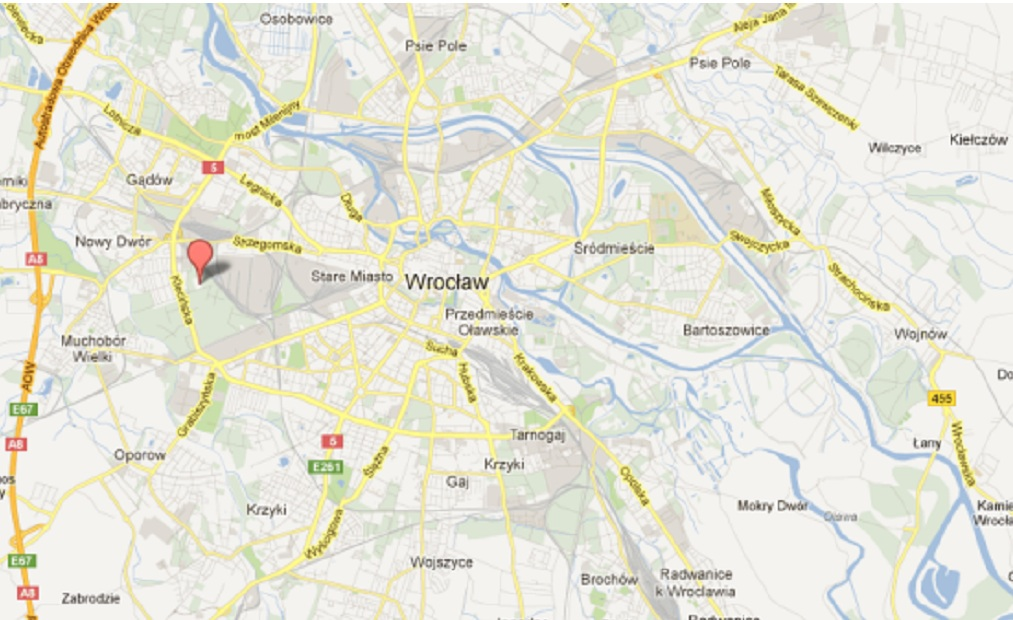
\includegraphics[width=0.8\textwidth]{./obrazki/adres_computerbudy.jpeg}
  \caption{Lokalizacja centrali firmy na mapie Wrocławia.}
\end{figure}

ComputerBudy jest firmą z działu IT. Zajmuje się ona zdalną pomocą przy problemach informatycznych. Zapewnia również zdalną administrację dla
skomplikowanych aplikacji na urządzeniach użytkownika. Jej oferta jest skierowana do osób prywatnych oraz małych i średnich firm, które
nie posiadają własnego działu IT.

Profil usług świadczonych powoduje, że brak połączenia z zewnętrzną siecią internet całkowicie paraliżuje całą firmę. 
Nawet awaria pojedynczego stanowiska powoduje straty. Restrykcyjna polityka bezpieczeństwa firmy sprawia, że nawiązanie połączenia z klientem
może nastąpić tylko z sieci firmowej. Aby zwiększyć bezpieczeństwo każde stanowisko obsługujące klientów jest przyłączone do sieci
za połączone za pomocą kabla UTP. Obostrzenia te spowodowane są obawą przed podsłuchaniem poufnych informacji przez osoby niepowołane oraz
przejęciem kontroli nad komputerem klienta podszywając się pod pracownika firmy z innej lokacji.

ComputerBudy wynajmuje łącznie 4 piętra w dwóch bliźniaczych budynkach stojących obok siebie.W pierwszym dwa i w następnym budynku kolejne dwa.
Pozostałe piętra wynajmują inne firmy.

Celem naszej pracy jest stworzenie projektu nowej instalacji teleinformatycznej na użytkowanych przez firmę piętrach w obu budynkach. Zakres projektu:
\begin{itemize}
\item{Inwentaryzacja sprzętu i infrastruktury dostępnej w przedsiębiorstwie}
\item{Analiza potrzeb użytkowników – wymagania zamawiającego}
\item{Założenia projektowe}
\item{Projekt sieci}
\subitem{Projekt logiczny sieci wraz z opisem koncepcji rozwiązania}
\subitem{Konfiguracja adresacji IP}
\subitem{Projekt okablowania}
\subitem{Projekt podłączenia do Internetu}
\subitem{Analiza bezpieczeństwa i niezawodności sieci}
\subitem{Kosztorys urządzeń}
 
\end{itemize}
Wnioskując z profilu usług firmy priorytetowe znaczenie podczas projektowania należy nadać niezawodności. Drugim w kolejności czynnikiem jest oczywiście
szeroko pojęte bezpieczeństwo. Wskazane jest również zapewnienie łatwej możliwości rozbudowy sieci w tym budynku na kolejne piętra.
Oczywiście jako, że zleceniodawca jest firmą prywatną należy zminimalizować koszty całego przedsięwzięcia.

Do stworzenia projektu instalacji teleinformatycznej zostaną użyte szczegółowe plany budynków udostępnione przez zleceniodawcę.
Wymagania użytkowników zostaną opracowane na podstawie danych przekazanych przez administratora IT firmy oraz poprzez konsultację
z samymi pracownikami. Przepustowości łącz w nowej instalacji zostaną oszacowane na podstawie danych z obecnie istniejącej sieci komputerowej.

\chapter{Inwentaryzacja sprzętu i infrastruktury dostępnej w przedsiębiorstwie}
Na podstawie udostępnionej dokumentacji oraz wizyt w budnyku mieszczącym firmę opracowano zestawienie zasobów obecnie posiadanych przez firmę.
W obecnej architekturze sieciowej razem w obu budynkach znajduje się 225 gniazdek ethernetowych. Całe obecne okablowanie wykonane jest 
za pomocą nieekranowanej skętki w kategorii 3. Jest to wyraźnie przestarzała technologia. W centrali znajduje się serwer realizujący usługę
bazy danych, serwera FTP oraz hostujący stronę internetową firmy. Serwer działa pod kontrolą systemu NetWare.

Wszystkie komputery PC oraz inne urządzenia przyłączone do sieci posiadają interfejsy sieciowe ethernet i spełaniają wymagania niezbędne
do połączenia do nowej sieci. Spis programów używanych w firmie:
\begin{enumerate}
 \item system operacyjny Windows XP
 \item przeglądarka Firefox
 \item program pocztowy Thundebird
 \item skype dla firm
 \item edytor tekstu Microsoft Office
 \item klient NetWare
 \item ssh
 \item TeamViever
 \item program księgowo kadrowy Płatnik
\end{enumerate}

Dodatkowo każdy dział ma dodatkowe oprogramowanie specyficzne dla funkcji jaką pełni. Specyfikacja ta zostanie sprecyzowana w następnym rozdziale.

Budynki w których firma ma swoją siedzibę to nowoczesne biurowce. Wynajmujący piętro sam zagospodarowuje większość 
znajdującej się tam przestrzeni za pomocą modułowej architektury boxów. Aby umożliwić dużą elestyczność konfiguracji przestrzennej piętra 
wyposażone są w podwieszane sufity w których poprowadzono jest większość instalacji. Właśnie pod kątem tego montażu zostanie zaprojektowany plan
okablowania.

Sieć energetyczna zainstalowana w budynku spełnia wszelkie wymagania dotyczące bezpieczeństwa oraz wydajności wymaganej dla sieci komputerowej.
Warte odnotowania jest obeność instalacji piorunochronowej na obu budynkach. Znacząco zwiększa to bezpieczeństow sprzętów elektronicznych zainstalowanych
w budynku.

Zakłócenia elektomagnetyczne w budyku są na tyle małe, że można je pominąć. W okolicy nie pracuje żaden duży zakaład przemysłowy, który mógłby 
znacząco wpłynąć na parametry zasilania w sieci. Inne firmy, które prowadzą swoją działalność w tych budynkach korzystają jedynie z standardowego
sprzętu birurowego połączonego kablową siecią ethernetową. Brak innych sieci bezprzewodowych w budynkach znacząco ułatwia implementacje sieci wifi
ponieważ nie występuje problem interferencji międzykanałowych.

%Trzba dodać orientacyjne oszacowanie ilości sprzętu.

%Z umieszczeniem tych planów to trzeba się jeszcze zastanowić.
\pagebreak[4]
Plany budynków znajdują się w załączniku A. Wzajemne rozmieszczenie budynków przezentuje poniższy rysunek.

%rysunek trzba poprawić
\begin{figure}[h!]
  \centering
      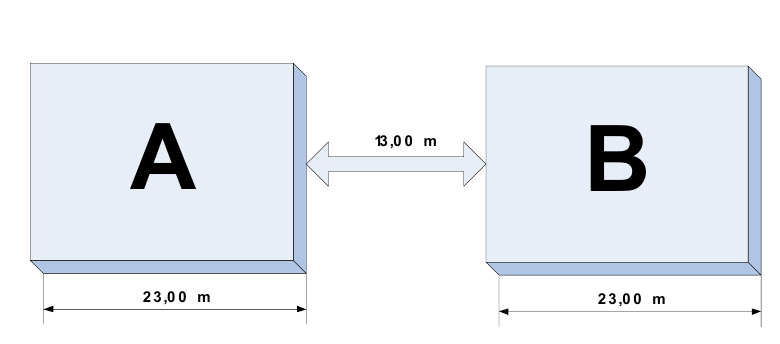
\includegraphics[width=0.8\textwidth]{./obrazki/rozmieszczenie_budynkow.jpeg}
  \caption{Wzajemne rozmieszczenie budynków.}
\end{figure}



\chapter{Analiza potrzeb użytkowników – wymagania zamawiającego}
Na podstawie danych dostarczonych przez administratora obecnej sieci powstała analiza wykorzystania łącz. Przedstawiają ją poniższe tabele:

%tabele

Wszyscy użytkowicy sieci korzystają z następujących programów: klient NetWare,Thundebird, Firefox, Microsoft Office oraz skype. Dodatkowo występuje 
oprogramowanie specjalistyczne dla wyszczególnionych działów. Księgowość i kadry pracują dużo na Płatniku natomiast obsługa klienta używa programu
do zdalenego zarządzania innymi komputerami TeamViever oraz ssh.

Firama w najbliższym czasie planuje zakup dodatkowych 4 drukarek siecowych.Po jednej dodatkowej na każde piętro.
W związku tymi planami należy zwiększyć liczbę gniazdek ethenetowych w instalacji do 229.

Firma w swojej bazie danych posiada nie tylko dane personalne swoich pracowników ale również klucze kryptograficzne wymagane do połączenia zdlanego
z maszyną klienta. Dane te są newralgiczne dla firmy. W związku z tym trzeba będzie w sieci koniecznie zastosować urządzenie typu firewall.

Serwer na którym jest umieszczona strona firmy do poprawnego obsługiwania zapytań potrzebuje łącze o przpustowośći 0,5 Mb/s do pobierania oraz
1 Mb/s do wysyłania. Wartości te będą uwzględnione dla wymagań dotyczących łącza internetowego.

Codziennie od godziny 24:00 do 6:00 rano wykonywany jest backup bazy danych klientów. Aby został poprawnie wykonany wymagana jest przepustowość 
na poziomie 3 Mb/s. Ponieważ czynność ta wykonywana jest w nocy wymaganie to będzie na pewno spełnione gdyż pracownicy nie będą generować ruchu
sieciowego.

Klient wyraził zapotrzbowanie na instalację sieci wifi dla działu obsługującego przetsiębiorców. W sali konferencyjnej często dochodzi  
do spotkań z klientami oraz małych narad zarządu. Wygodny dostęp dla intenetu na pewno byłby czynnikiem ułatwiającym wszelkie negocjacje.
Niestety nie można przewidzieć zapotrzebowania na pasmo dla tego elementu sieci ponieważ nie wiadomo jaki program zechce uruchomić użytkownik.
Nie jest to obciążenie ciągłe sieci więc odpowiedni zapas przepustowości w powinien rozwiązać ten problem.

Na podstawie zebranych danych można postawić wymagania dotyczące przpustowości sieci lokalnej oraz łącza z intenetowego. Poniższa tabela
prezentuje wymagania minimalne oraz zalecane. Wymagania minimalne zawierają wartości parametrów niezbędych do poprawnego działania sieci. 
Niestety gdyby ich użyć mogłyby wystąpić problemy z jakością usług gdyby jakiś program przeciążył sieć. Aby tego uniknąć należy użyć wartośći
zalecanych, które stanowią trzykrotność wartości minimalnej. Z takim zapasem przepustowości sieć będzie odporana na większość przeciążeń.

%tabelka


\chapter{Założenia projektowe}
\chapter{Projekt sieci}
\section{Projekt logiczny sieci wraz z opisem koncepcji rozwiązania}
\section{Konfiguracja adresacji IP}
\section{Projekt okablowania}
\section{Projekt podłączenia do Internetu}
\section{Analiza bezpieczeństwa i niezawodności sieci}
\section{Kosztorys urządzeń}

%Otoczenie tabelki
%\begin{table}
 % \caption{Geograficzne rozmieszczenie odziałów firmy.}
 %\includegraphics[width=0.9\textwidth]{./obrazki/topologia.jpeg}
%\end{table}

%\begin{figure}[h!]
 % \centering
 %     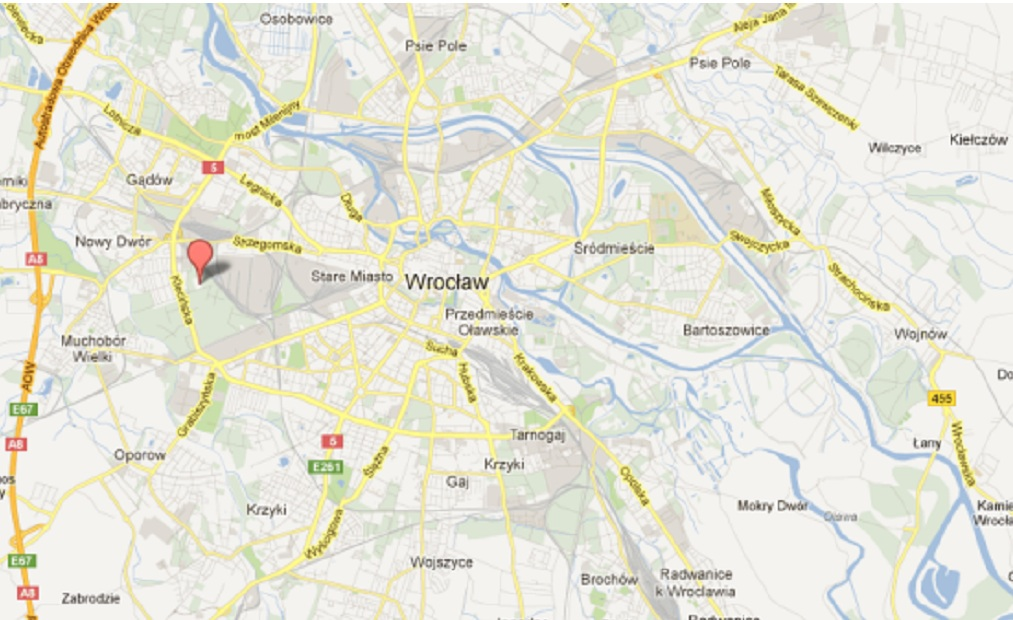
\includegraphics[width=0.9\textwidth]{./obrazki/adres_computerbudy.jpeg}
%  \caption{Geograficzne rozmieszczenie odziałów firmy.}
%\end{figure}

%\chapter*{notatki}


\end{document}
